% Matteo Kumar - Leonard Schatt
% Physikalisches Praktikum

% Anhang A

\chapter{Anhang}
\section{Absorbtionskoeffizient}

\begin{figure}[ht]
    \centering
    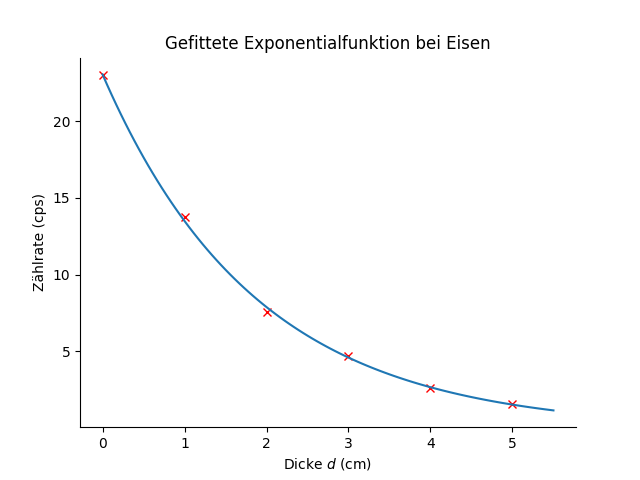
\includegraphics[width = 12cm]{Bilder/Auswertung/AbsorbtioskFe.png}
    \caption{Zählrate bei jeweiliger Absorberdicke $d$}
    \label{AbsorbtionkoeffFe}
\end{figure}


\begin{figure}[ht]
    \centering
    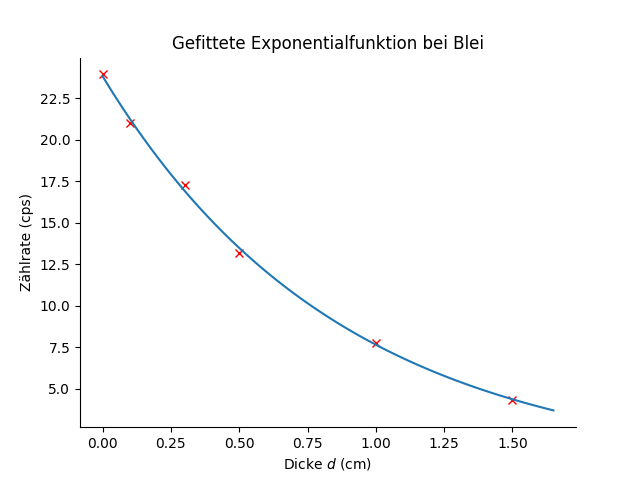
\includegraphics[width = 12cm]{Bilder/Auswertung/AbsorbtioskPb.png}
    \caption{Zählrate bei jeweiliger Absorberdicke $d$}
    \label{AbsorbtionkoeffPb}
\end{figure}



\clearpage
\section{Daten}
Die gemessene Rohdaten könne unter folgendem Link eingesehen werden:\\
\url{https://1drv.ms/u/s!Ap8DY8lEb1DBwH4yWeWRU46oaMHg?e=fMecIw}
